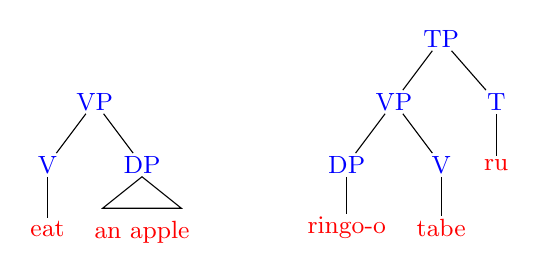
\begin{tikzpicture}[c/.style={blue, font=\small, inner sep=1pt}, wd/.style={red, font=\small, inner sep=1pt}]
% English (head-initial): [VP [V eat] [DP an apple]]
\node[c] (VP) at (1,0) {VP};
\node[c] (V) at (0.4,-0.8) {V};
\node[c] (DP) at (1.6,-0.8) {DP};
\node[wd, anchor=north] (eat) at (0.4,-1.47) {eat};
\node[wd, anchor=north] (apple) at (1.6,-1.47) {an apple};
\draw (VP) -- (V); \draw (VP) -- (DP); \draw (V) -- (eat);
\draw (DP.south) -- ++(-0.5,-0.4) -- ++(1.0,0) -- cycle;
% Japanese (head-final): [TP [VP [DP ringo-o] [V tabe]] [T ru]]
\begin{scope}[xshift=4cm, yshift=0.8cm]
\node[c] (TP) at (1.4,0) {TP};
\node[c] (VP) at (0.8,-0.8) {VP};
\node[c] (T) at (2.1,-0.8) {T};
\node[c] (DP) at (0.2,-1.6) {DP};
\node[c] (V) at (1.4,-1.6) {V};
\node[wd] (ringo) at (0.2,-2.4) {ringo-o};
\node[wd] (tabe) at (1.4,-2.4) {tabe};
\node[wd] (ru) at (2.1,-1.6) {ru};
\draw (TP) -- (VP); \draw (TP) -- (T); \draw (T) -- (ru);
\draw (VP) -- (DP); \draw (VP) -- (V);
\draw (DP) -- (ringo); \draw (V) -- (tabe);
\end{scope}
\end{tikzpicture}
